
\chapter{Ejercicios y soluciones}

\section{Boletín 1:} \label{Sec:Ej-01}

\subsection{Ejercicios}
\tcbstartrecording

\begin{texercise}
    Encuentra dos ejemplos de triplete de isoespín, otro ejemplo de ``cuatriplete'', y otro de ``quintuplete'' en núcleos ligeros. Discute las diferencias de energía entre los estados análogos de isoespín de cada grupo e intenta dar una configuración de nucleones que explique sus estructuras.
\tcblower
    Los estados triplete de isoespín son aquellos que tienen $T=1$, los estados cuatripletes son aquellos con $T=3/2$ y los quintupletes con $T=2$. Por ejemplo el carbono 10 tiene $Z=6$ y $N=4$ 
\end{texercise}

\begin{texercise}
    Comprueba si la interacción de Skyrme cumple las simetrías subyacentes de la fuerza nuclear.
\tcblower
    Las simetrías subyacentes a la fuerza nuclear, como bien sabemos (véase \cref{Subsec:02-01-03} para mayor explicación): 

    \begin{itemize}
        \item Invarianza traslacional: las dependencias deben corresponder a la distancia relativa $\rn=\rn_1-\rn_2$.
        \item Invarianza de Loretz: la interacción debe ser la misma para cualquier sistema de referencia inercial, y por tanto la dependencia con el momento debe ser también relativa $\pn=\pn_1-\pn_2$.
        \item Invarianza rotacional: todos los términos de la intearcción deben tener un momento angular total nulo.
        \item Invarianza de iesoespín. La interacción debe ser isoescalar en el espacio de isoespín: solo términos $(\tau_1\cdot\tau_2)^n$ deben estar permitidos. 
        \item Invarianza de paridad: los términos con $\rn$ y $\pn$ deben tener potencias pares. 
        \item Invarianza de inversión teporal: los términos con $\pn$ y espín $\sigma$ deben tener potencias pares. 
    \end{itemize}
    Ahora solo tenemos que ver que la interacción de Skyrme no posee las diferentes dependencias prohibidas (distancias no relativas, términos de momento angular...) o aplicar invarianza de paridad/temporal (la invairanza de paridad es $\rn\rightarrow -\rn$ y la temporal $t\rightarrow -t$). La itneracción de Skyrme
\end{texercise}

\begin{texercise}
    Demuestra que los estados permitidos en el acoplamiento de tres fonones cuadrupolares son $0^+$, $2^+$, $3^+$, $4^+$, y $6^+$.
\tcblower
    Queremos acoplar tres fonones cuadrupolares, es decir, queremos hacer un acoplamiento $2\oplus 2\oplus 2$. Lógicamente la paridad va a ser positiva, ya que 

    \begin{equation}
        \pi = (-)^2 (-)^2 (-)^2 = +
    \end{equation}
    Ahora solo resta acoplar los modos de vibración. Esto exige un acoplamiento un tanto diferente al habitual. Primero usamos el acoplamiento de $2\oplus 2$ dado por los apuntes, que nos dice que 

    \begin{equation*}
        2 \oplus 2 = 0^+,1^-,2^+,,4^+
    \end{equation*}
    
\end{texercise}

%%%%%%%%%%%%%%%%%%%%%%%%%%%%%%%%%%%%%%%%%%%
%%%%%%%%%%%%%%%%%%%%%%%%%%%%%%%%%%%%%%%%%%%
%%%%%%%%%%%%%%%%% EJERCICIO 1.4 %%%%%%%%%%%
%%%%%%%%%%%%%%%%%%%%%%%%%%%%%%%%%%%%%%%%%%%
%%%%%%%%%%%%%%%%%%%%%%%%%%%%%%%%%%%%%%%%%%%

\begin{texercise}
    Encuentra los posibles estados (espín y paridad) que resultarían del acoplamiento de un fonón cuadrupolar y un octupolar.
\tcblower
    Todavía no está redactado. 
\end{texercise}

%%%%%%%%%%%%%%%%%%%%%%%%%%%%%%%%%%%%%%%%%%%
%%%%%%%%%%%%%%%%%%%%%%%%%%%%%%%%%%%%%%%%%%%
%%%%%%%%%%%%%%%%% EJERCICIO 1.5 %%%%%%%%%%%
%%%%%%%%%%%%%%%%%%%%%%%%%%%%%%%%%%%%%%%%%%%
%%%%%%%%%%%%%%%%%%%%%%%%%%%%%%%%%%%%%%%%%%%


\begin{texercise}
    \textbf{Ejercicio 5}
    El núcleo de $^{68}$Er tiene su primer estado excitado 2+ en 91.4 keV.
    \begin{enumerate}
        \item Sabiendo que es el primer estado de una banda rotacional, determina su momento de inercia.
        \item ¿Cuáles serían las energías de los siguientes cuatro estados de la misma banda? Compara con los valores experimentales (208.1, 315.0, 410.2, 493.5 keV).
    \end{enumerate}
\tcblower
Todavía no está redactado.
\end{texercise}


%%%%%%%%%%%%%%%%%%%%%%%%%%%%%%%%%%%%%%%%%%%
%%%%%%%%%%%%%%%%%%%%%%%%%%%%%%%%%%%%%%%%%%%
%%%%%%%%%%%%%%%%% EJERCICIO 1.6 %%%%%%%%%%%
%%%%%%%%%%%%%%%%%%%%%%%%%%%%%%%%%%%%%%%%%%%
%%%%%%%%%%%%%%%%%%%%%%%%%%%%%%%%%%%%%%%%%%%


\begin{texercise}
    \textbf{Ejercicio 6}
    ¿Por qué dos nucleones en la misma capa se acoplan sólo a $j$ pares ($j = 0, 2, 4, \dots$)?
\tcblower
    Porque minimizan la energía del apareamiento de nucleones.
\end{texercise}


%%%%%%%%%%%%%%%%%%%%%%%%%%%%%%%%%%%%%%%%%%%
%%%%%%%%%%%%%%%%%%%%%%%%%%%%%%%%%%%%%%%%%%%
%%%%%%%%%%%%%%%%% EJERCICIO 1.7 %%%%%%%%%%%
%%%%%%%%%%%%%%%%%%%%%%%%%%%%%%%%%%%%%%%%%%%
%%%%%%%%%%%%%%%%%%%%%%%%%%%%%%%%%%%%%%%%%%%


\begin{texercise}
    \textbf{Ejercicio 7}
    \begin{enumerate}
        \item Construye la línea yrast de dos núcleos con $A>150$ y otros dos con $A<100$.
        \item Deduce el momento de inercia en función del cuadrado de la frecuencia de rotación y discute la aparición de backbending e identifica las diferentes bandas rotacionales.
        \item Compara los resultados con lo esperado en un sólido rígido y un fluido sin viscosidad.
        \item En los núcleos con $A<100$, intenta identificar bandas vibracionales.
    \end{enumerate}
\tcblower
    \textbf{Apartado a)}.  Primero tenemos que definir qué es la línea \textit{yrast} para poder constuirla. La línea yrast es la trayectoria que conecta, en un diagrama de energía versus espín, los estados con la energía de excitación más baja para cada valor de momento angular $I$ (espín) en un núcleo. Es decir, para cada espín $I$, el estado yrast es el de mínima energía, y estos estados resultan ser los más favorecidos en la formación de bandas rotacionales. Nos piden los bandas yrast de 4 átomos, 2 para $A<100$ y 2 para $A>150$. Los elegidos son: $^{84}$Zr, $^{86}$Zr, $^{160}$Eu, $^{156}$Eu. Los motivos por los que son elegidos es que presentan una gran cantidad de datos en el nndc, además de que son núcleos par-par, que al tener como primer estado fundamental $0^+$ obliga a que las bandas rotacionales estén compuestos de estados con $I$ par de paridad positiva ($4^+,6^+,8^+...$). Esto es intersante ya que facilita la recolección de datos de la nndc. 

    Lo primero que hacemos es entrar en la lista de niveles de la nndc (\textit{list of levels}) y elegir los que, para los estados $2^+,4^+...$ tienen el valor de energía más pequeño. En principio no nos vamos a fijar en nada más, ya que así es la definición de la línea Yrast. Es posible que existan estados con valores $14^+$ que no pertecenzcan a bandas rotacionales (siendo excitacioens de partículas individuales), pero esto debería ser detectable en la propia gráfica del yrast, y mencionado posteriormente. Así pues, las líneas yrast son: 

    \begin{center}
        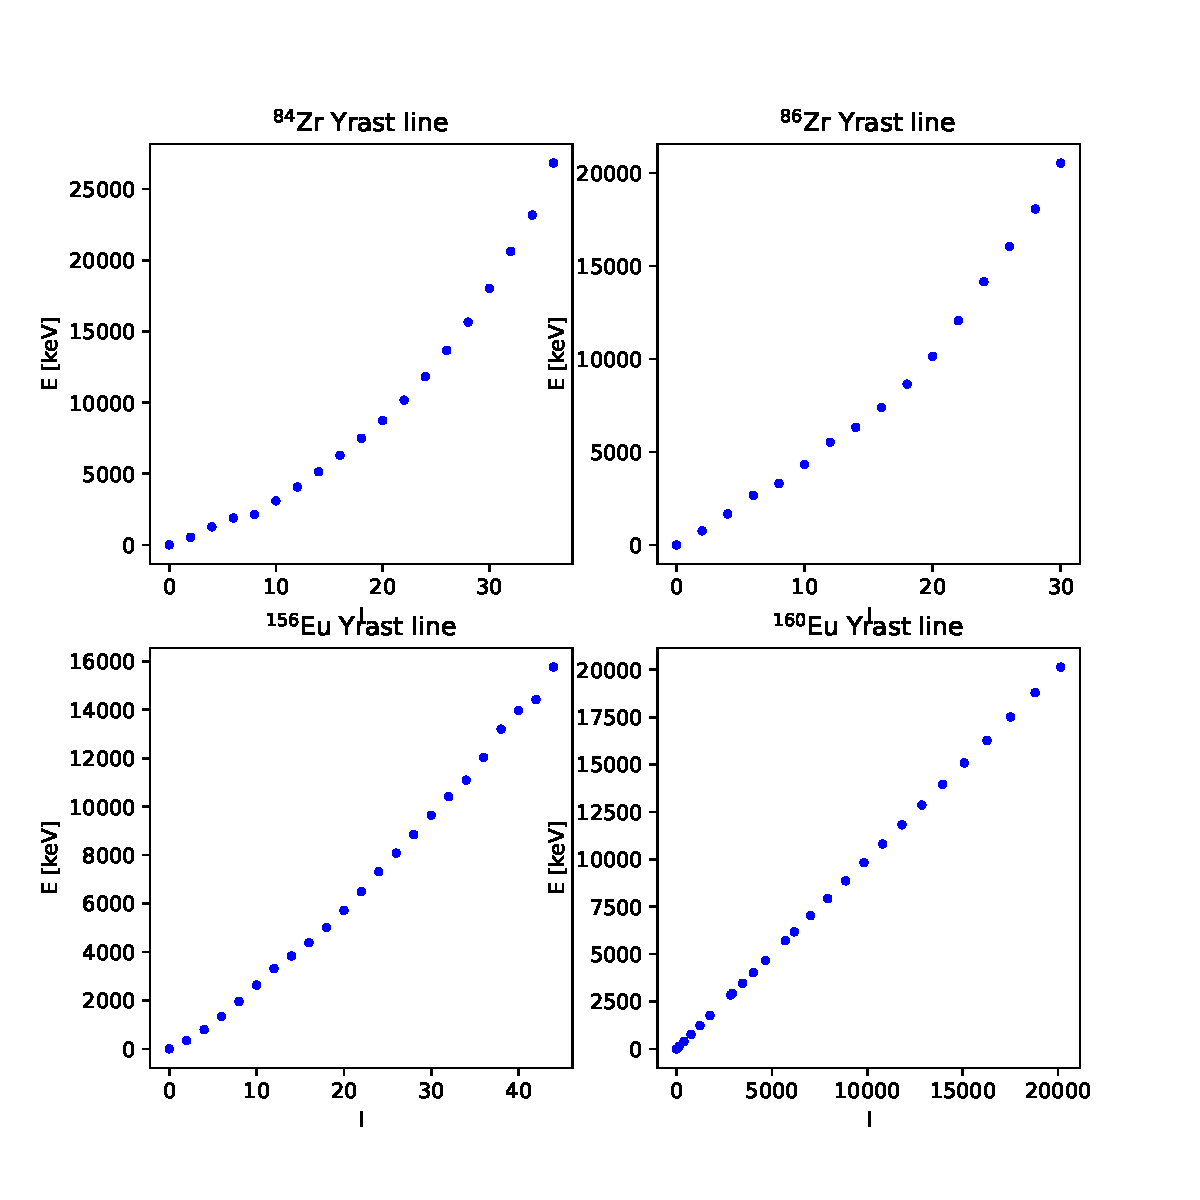
\includegraphics[width=0.8\linewidth]{Cuerpo/Boletin_01/Yrast_total.pdf}
    \end{center}

    Como podemos ver las líneas del circonio están bastante bien, cuadrando en un esquema $E \propto I(I+1)$. Sin embargo las líneas de los europios son bastante malas, en particular la del europio 160, es prácticamente una línea recta. Lo más probable es que efectivamente hallamos colocado estados de excitación individual, excitación vibracional u otros fenómenos que no correspondan a una banda rotacional. Si nos sobra tiempo incluiremos al final del ejercicio una serie de datos corregidos que podrían pertenecer a diferntes bandas rotacionales, o quizás incluyamos un núcleo con mejor resultado. 

   % \begin{center}
   %     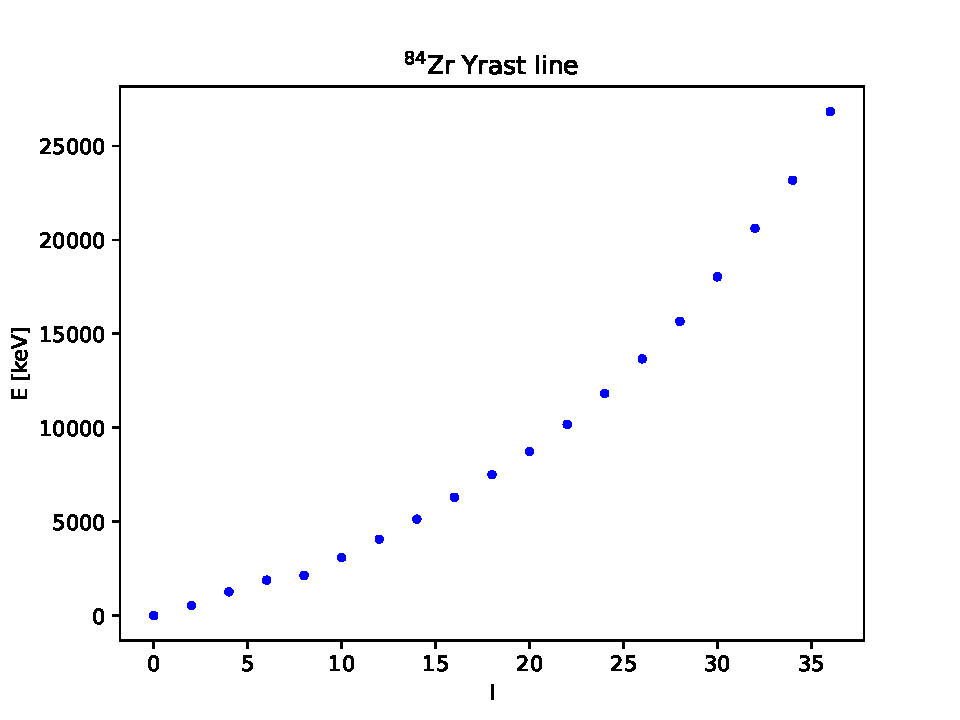
\includegraphics[width=0.8\linewidth]{Cuerpo/Boletin_01/Yrast_Zr84.pdf}
   % \end{center}
   % \begin{center}
   %     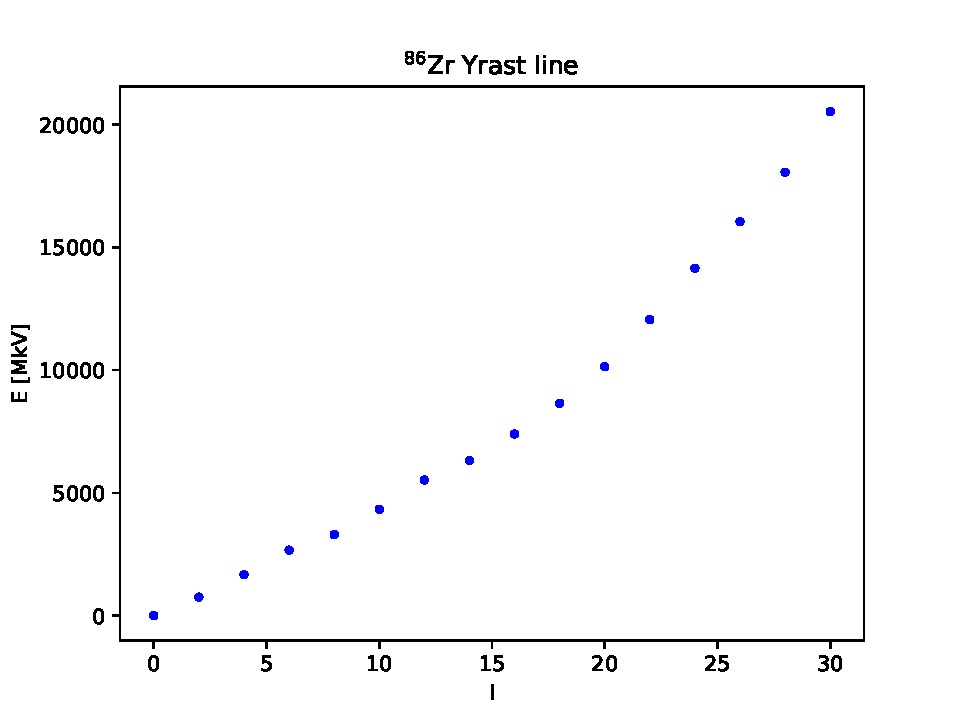
\includegraphics[width=0.8\linewidth]{Cuerpo/Boletin_01/Yrast_Zr86.pdf}
   % \end{center}
   % \begin{center}
   %     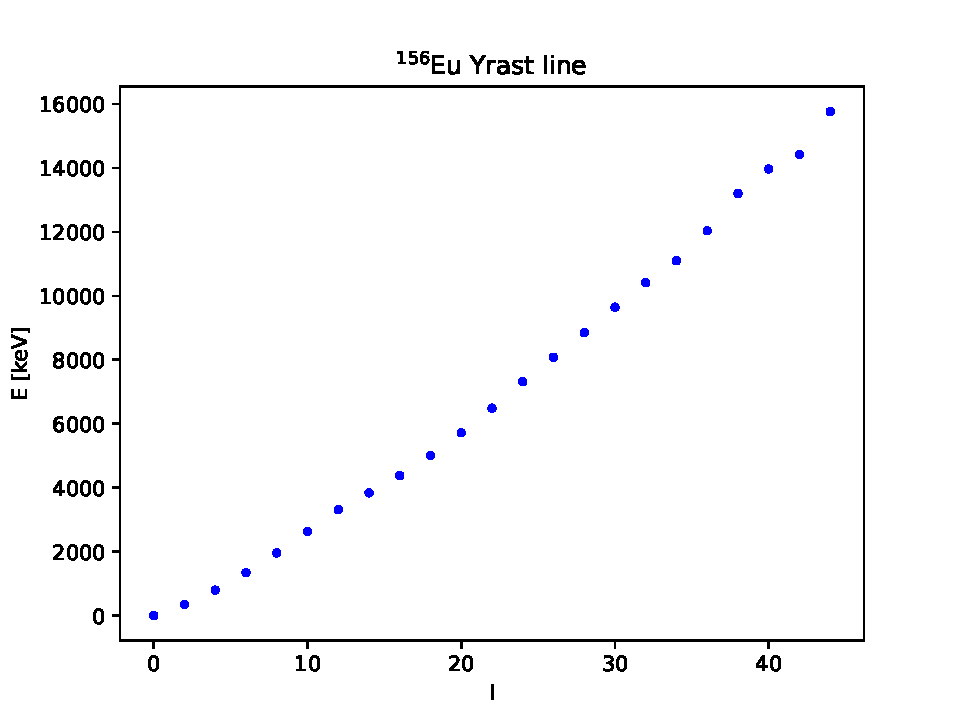
\includegraphics[width=0.8\linewidth]{Cuerpo/Boletin_01/Yrast_Eu156.pdf}
   % \end{center}
   % \begin{center}
   %     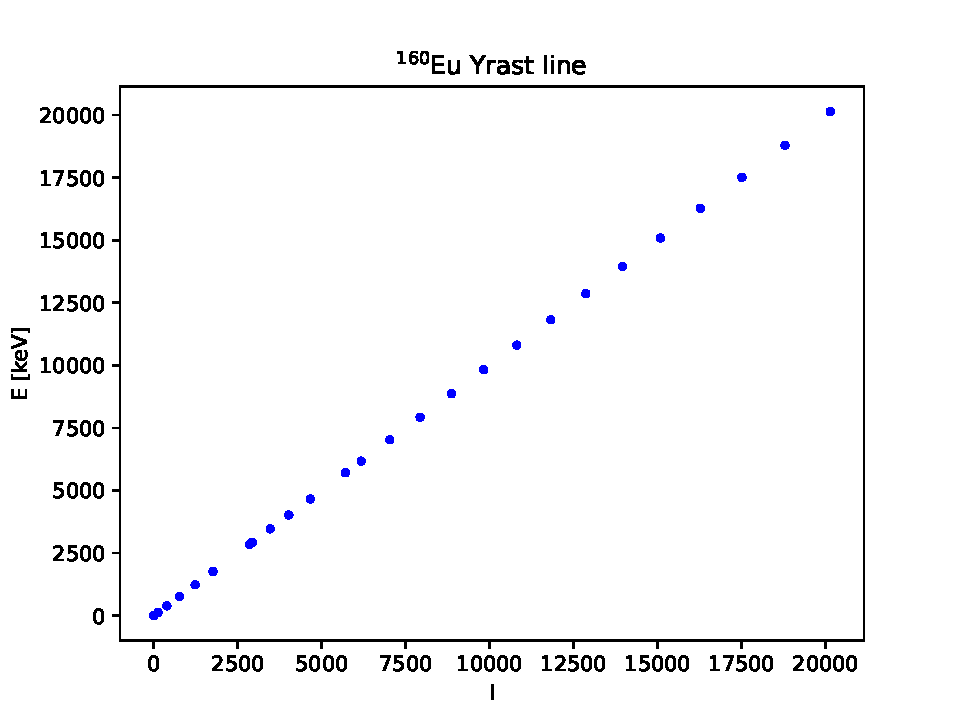
\includegraphics[width=0.8\linewidth]{Cuerpo/Boletin_01/Yrast_Eu160.pdf}
   % \end{center}

    \textbf{Apartado b)} Ahora tenemos que calcular el momento de inercia en función de la frecuencia de rotación, discutiendo la aparición del backbending. Para calcular el momento de intercia en función de frecuencia $\omega$ primero necesitamos una $\omega$, que se obtiene de la siguiente fórmula:

    \begin{equation}
        \hbar \omega =  \frac{E_{I}-E_{I-2}}{\ccorchetes{I(I+1)}^{1/2}-\ccorchetes{(I-2)(I-1)}^{1/2}} \approx \frac{E_I-E_{I-2}}{2}
    \end{equation}
    que sacamos del libro \textit{Shape and Shells in Nuclear Structura} de \textit{Nilsson y Ragnarsson}, aunque la última aproximación ya se encontraba en las diapositivas. También sabemos que el momento de inercia $\Ical$ se relaciona con nuestra energía de rotación  y momento de inercia como:

    \begin{equation}
        E_{I} = \frac{\hbar^2}{2\Ical} \ccorchetes{I(I+1)}
    \end{equation}
    para núcleos par-par donde $K=0$. Entonces podemos ver que para un $E_I$ dado podemos asignar un $\hbar \omega$ (ya que $E_0=0$) y para cada $E_I$ dado podemos calcualr $2I/\hbar^2$, tal que:
    
    \begin{equation}
       \frac{2\Ical}{\hbar^2} = \frac{I(I+1)}{2E_I}
    \end{equation}
    Lógicamente lo vamos a realizar en python, tal que las gráficas obtenidas resultan:

    \begin{center}
        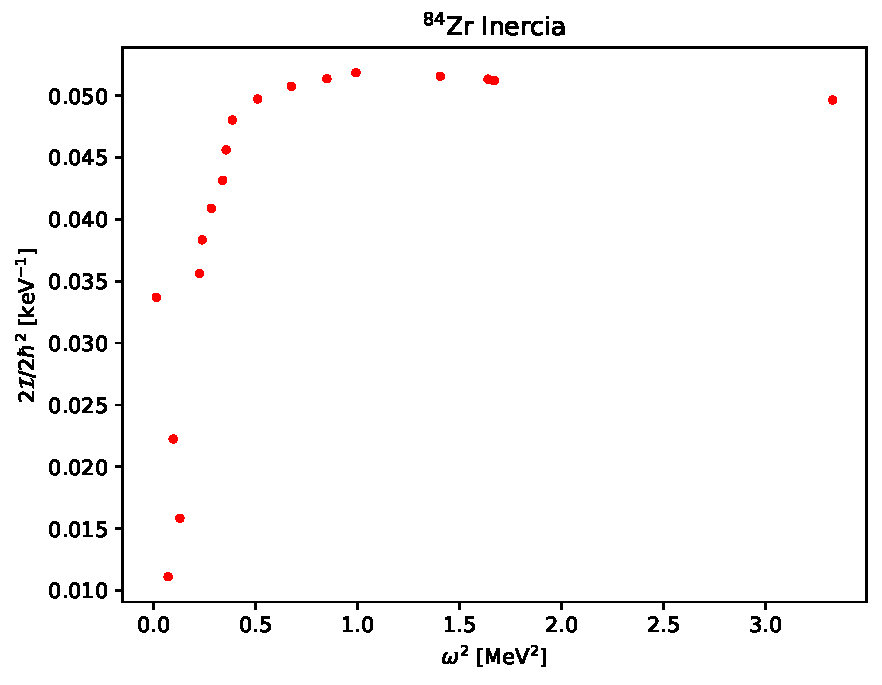
\includegraphics[width=0.6\linewidth]{Cuerpo/Boletin_01/84Zr_inercia.pdf}
    \end{center}
    \begin{center}
        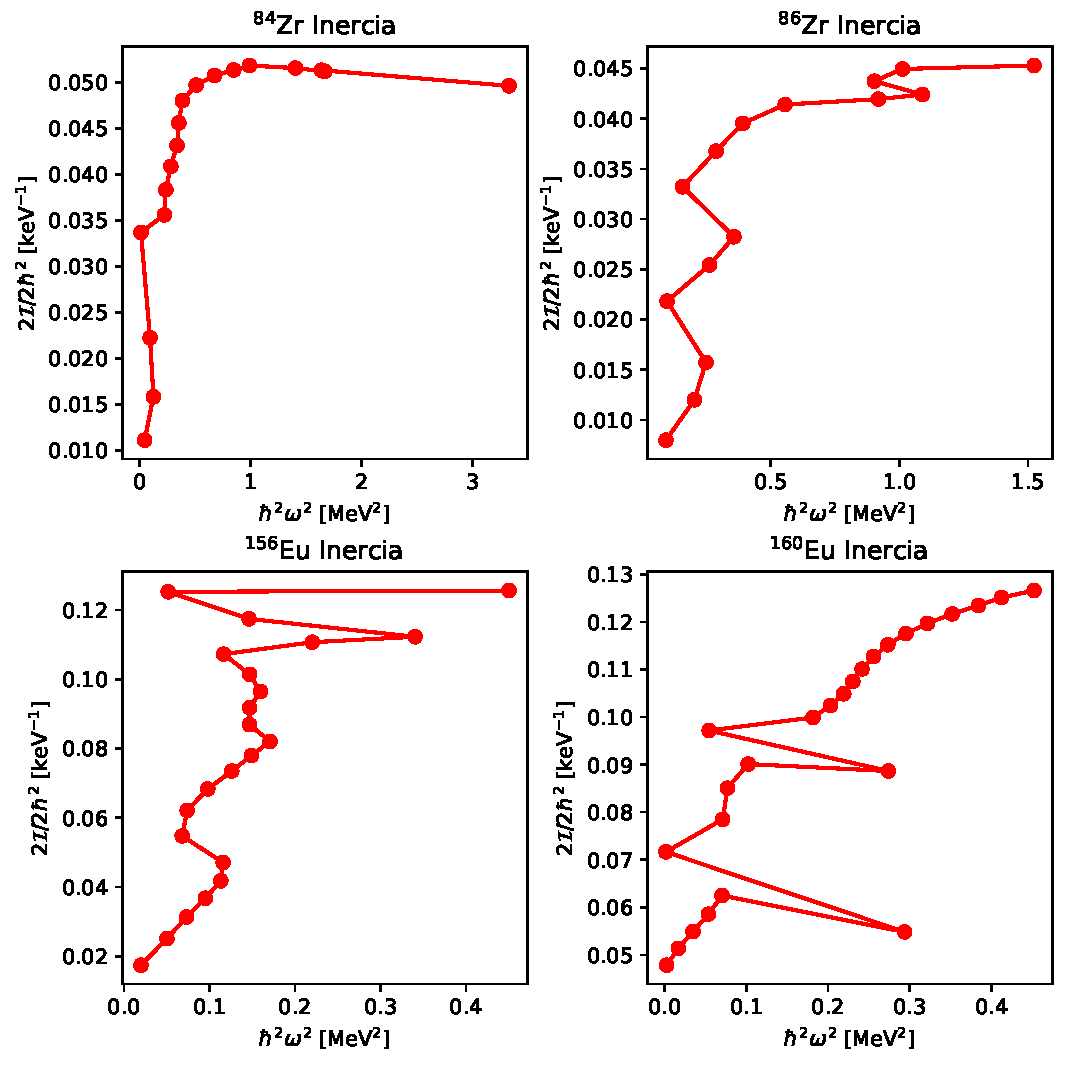
\includegraphics[width=0.6\linewidth]{Cuerpo/Boletin_01/86Zr_inercia.pdf}
    \end{center}
    \begin{center}
        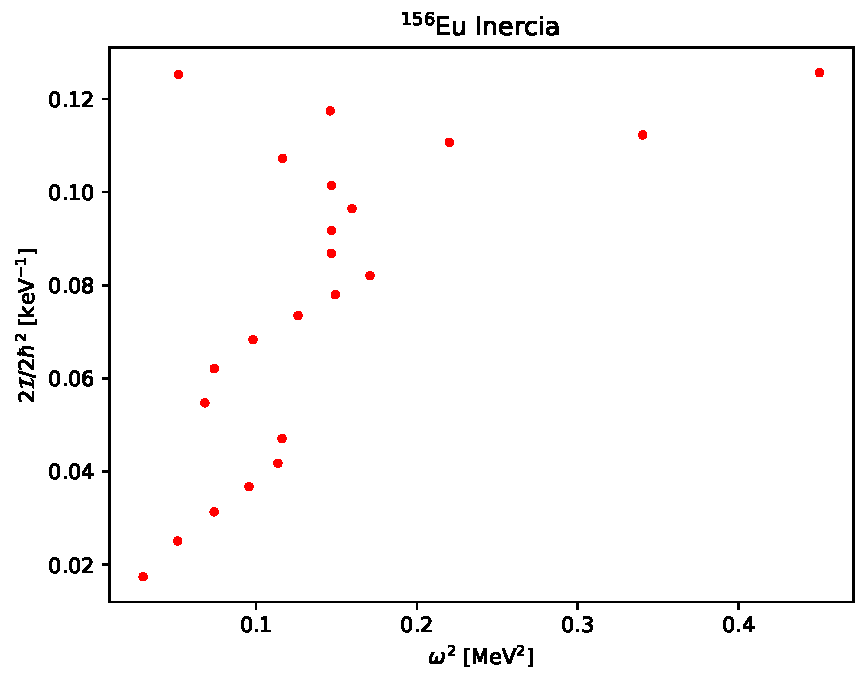
\includegraphics[width=0.6\linewidth]{Cuerpo/Boletin_01/156Eu_inercia.pdf}
    \end{center}
    \begin{center}
        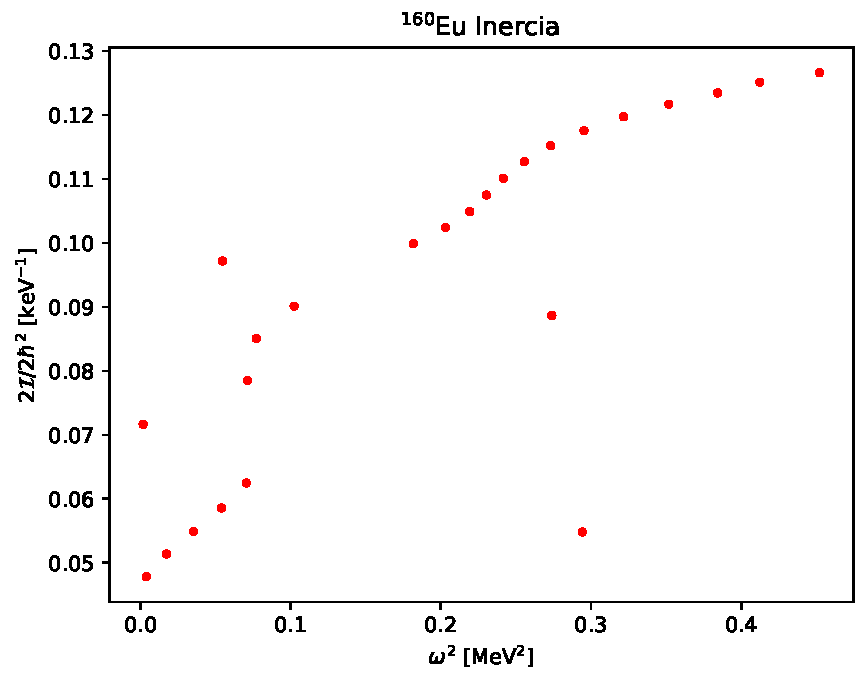
\includegraphics[width=0.6\linewidth]{Cuerpo/Boletin_01/160Eu_inercia.pdf}
    \end{center}
    Como podemos ver en ninguno de los casos nos aparece algo como $\Ical = \alpha \omega^2$ (que en las gráficas se representaría como una línea recta). En todos los casos hay un comportamiento  inicial a la cuarta con la frecuencia $\Ical \propto \omega^4$, apareciendo backbending inmediato tanto en los núcleos ligeros como en los núcleos pesados, como en los núcleos ligeros.

    Aunque es probable que algunos de los datos estén mal cogidos y realmente no pertenezcan a una de las bandas rotacionales, la inercia se enfrenta a la frecuencia tal y como esperabamos: de manera que aparecen zonas con cierta similitud (bandas rotacionales) que se disgregan rápidamente. Las bandas rotacionales se pueden detectar tanto en la línea yrast como en el backbending, aunque es mucho más facil de detectar en las líneas Yrast:


    \begin{center}
        \includegraphics[width=0.55\linewidth]{Cuerpo/Boletin_01/Yrast_total_parabolic.pdf}
    \end{center}

    Como podemos ver, tanto para el $^{86}$Zr, $^{156}$Eu y $^{160}$Eu la aproximación de una banda rotacinal es bastante mala, mientras que para el $^{84}$Zr está bien, de hecho hemos probado varias versiones y no hemos conseguido una mejor representación entre varias bandas.

    \begin{center}
        \includegraphics[width=0.55\linewidth]{Cuerpo/Boletin_01/Yrast_total_parabolic2.pdf}
    \end{center}






\end{texercise}


%%%%%%%%%%%%%%%%%%%%%%%%%%%%%%%%%%%%%%%%%%%
%%%%%%%%%%%%%%%%%%%%%%%%%%%%%%%%%%%%%%%%%%%
%%%%%%%%%%%%%%%%% EJERCICIO 1.8 %%%%%%%%%%%
%%%%%%%%%%%%%%%%%%%%%%%%%%%%%%%%%%%%%%%%%%%
%%%%%%%%%%%%%%%%%%%%%%%%%%%%%%%%%%%%%%%%%%%


\begin{texercise}
    \textbf{Ejercicio 8}
    Usando el esquema de niveles tradicional del modelo de capas mostrado en la tabla 1,
    \begin{enumerate}
        \item Calcula la corrección de Strutinsky (sin incluir apareamiento) para $Z=50, N=82$ y para $Z=40, N=68$.
        \item Estudia el resultado en función de la anchura $\gamma$ de la Gaussiana.
    \end{enumerate}
\tcblower
    \begin{center}
        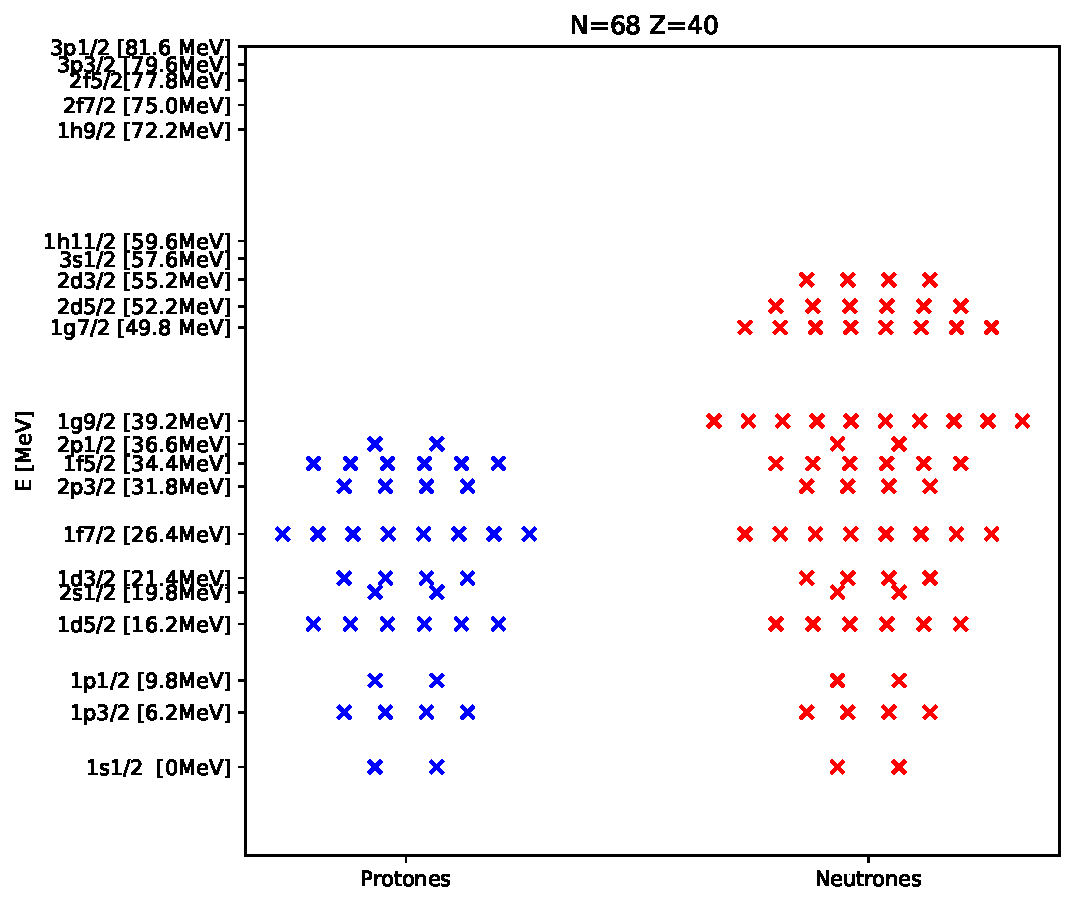
\includegraphics[width=0.6\linewidth]{Cuerpo/Boletin_01/N68_Z40_Bandas.pdf}
    \end{center}
    \begin{center}
        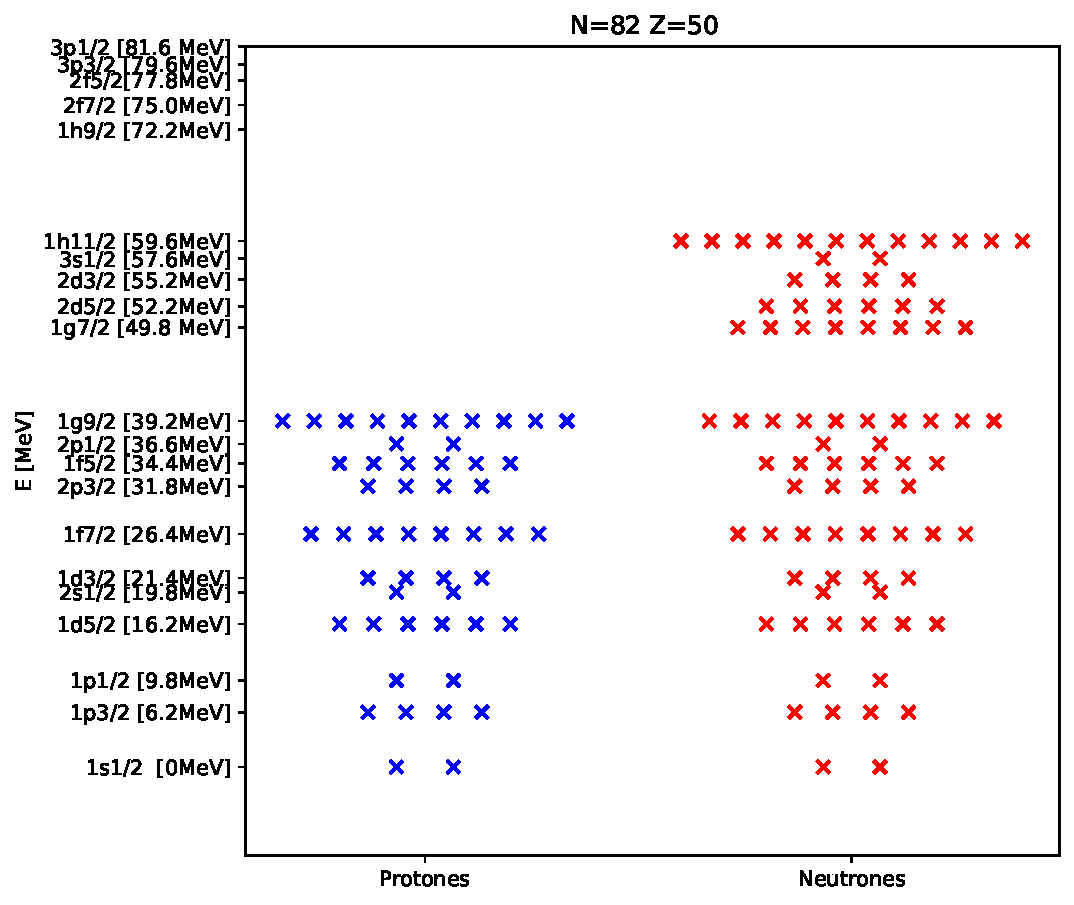
\includegraphics[width=0.6\linewidth]{Cuerpo/Boletin_01/N82_Z50_Bandas.pdf}
    \end{center}
    \begin{center}
        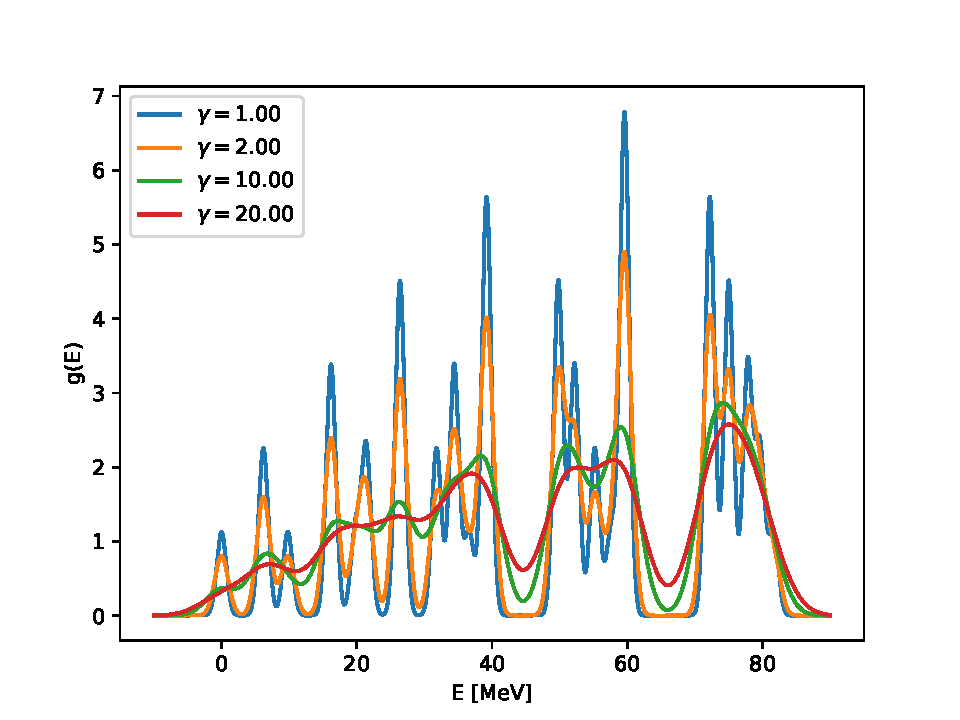
\includegraphics[width=0.6\linewidth]{Cuerpo/Boletin_01/ge.pdf}
    \end{center}
\end{texercise}


\tcbstoprecording


\subsection{Solucion}
\tcbinputrecords